% !TeX program = pdflatex
% !TeX encoding = utf8
% !TeX spellcheck = uk_UA
% !BIB program = bibtex8

\documentclass[18pt]{LectMechanics}

\usetikzlibrary{arrows.meta}

\title[Physics 1]{\huge\bfseries Rotational motion of a point and its angular characteristics. Kinematics of a rigid body}
\date{}

\begin{document}
%=======================================================================================================
%\usebackgroundtemplate{
%
%\tikz\node[opacity=0.3]{\includegraphics[width=\paperwidth,height=\paperheight]{background}};%
%}
\begin{frame}
	\titlepage
\end{frame}
%=======================================================================================================
\usebackgroundtemplate{
}




%=======================================================================================================
\begin{frame}{Goals for Lecture}{}
	\begin{itemize}
		\item To determine what is angular position
		\item To determine what is angular displacement
		\item To determine what is angular velocity
		\item To determine what is angular acceleration
		\item To describe the rotational motion under constant angular acceleration
		\item To understand what is  relations between angular and linear quantities
		\item To describe the circular motion of a particle
	\end{itemize}
\end{frame}
%=======================================================================================================


%=======================================================================================================
\begin{frame}{Angle and Radian}{}
	\begin{columns}
		\begin{column}{0.5\linewidth}
			\begin{enumerate}
				\item $\phi$ can be defined as the arc length $s$ along a circle divided by the radius $r$:
				\item The angular position, measured in radians, is the angle of rotation of the object with respect to a reference position.
				\item The angular position of point $A$ at this point in time is equal to $\phi$.  In order to uniquely define this position, we have assume that an the angular position is measured with respect to the $x$ axis.
			\end{enumerate}
		\end{column}
		\begin{column}{0.5\linewidth}
			\begin{tikzpicture}
				\footnotesize
				\pgfmathsetmacro{\R}{1.5}
				\pgfmathsetmacro{\ang}{45}
				\draw[step=0.25, lightgray] (-2,-2) grid (2,2);
				\draw[-latex, thick] (0,-2.5) -- (0,2.5) node[left] {$y$};
				\draw[-latex, thick] (-2.5,0) -- (2.5,0) node[below] {$x$};
				\draw[thick, blue,
					decoration={markings, mark=at position 0.4/2 with \arrow{latex}},
					postaction=decorate
				] (0,0) circle (\R);
				\draw (0,0) -- node[above] {$r$} (\ang:\R) coordinate (A);
				\fill[red] (A) circle (0.05) node[above] {$A$};
				\draw[thick] (0,0) (0:\R/5) arc(0:\ang:\R/5) node[pos=0.7,right] {$\phi$};
				\draw[red, latex-latex] (0,0) (0:1.1*\R) arc(0:\ang:1.1*\R) node[pos=0.5, circle, above right=0.01pt] {$s$};
			\end{tikzpicture}
		\end{column}
	\end{columns}
\end{frame}
%=======================================================================================================

%=======================================================================================================
\begin{frame}{Angle and Angular Displacement}{}
	\begin{columns}
		\begin{column}{0.5\linewidth}
			Angular displacement $\Delta\phi = \phi_2 - \phi_1$
		\end{column}
		\begin{column}{0.5\linewidth}
			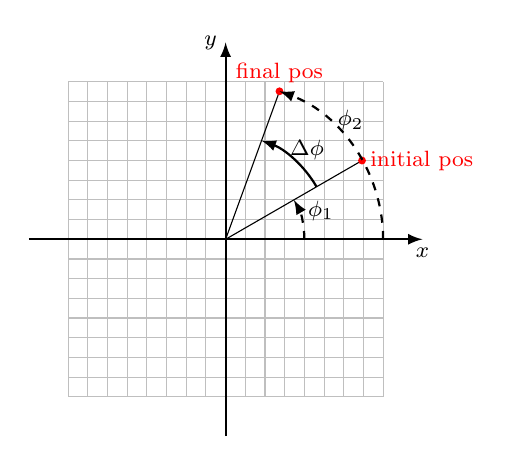
\begin{tikzpicture}
				\footnotesize
				\pgfmathsetmacro{\R}{2}
				\pgfmathsetmacro{\ang}{30}
				\draw[step=0.25, lightgray] (-2,-2) grid (2,2);
				\draw[-latex, thick] (0,-2.5) -- (0,2.5) node[left] {$y$};
				\draw[-latex, thick] (-2.5,0) -- (2.5,0) node[below] {$x$};
				%		\draw[thick, blue, , dash dot, 
				%		decoration={markings, mark=at position 0.6/2 with \arrow{latex}},
				%		postaction=decorate
				%		] (0,0) circle (\R);
				\draw (0,0) --  (\ang:\R) coordinate (A);
				\fill[red] (A) circle (0.05) node[right] {initial pos};
				\draw[thick, dashed, -latex] (0,0) (0:\R/2) arc(0:\ang:\R/2) node[pos=0.7,right] {$\phi_1$};

				\draw (0,0) -- (\ang+40:\R) coordinate (A);
				\fill[red] (A) circle (0.05) node[above] {final pos};
				\draw[thick, dashed, -latex] (0,0) (0:\R/1) arc(0:\ang+40:\R/1) node[pos=0.7,right] {$\phi_2$};

				\draw[thick, -latex] (0,0) (\ang:\R/1.5) arc(\ang:\ang+40:\R/1.5) node[pos=0.7,right] {$\Delta\phi$};
			\end{tikzpicture}
		\end{column}
	\end{columns}
\end{frame}
%=======================================================================================================


%=======================================================================================================
\begin{frame}{Angular Displacement}{Angular Displacement is VECTOR!}
	\begin{columns}
		\begin{column}{0.5\linewidth}
			\begin{overprint}
				\onslide<1>
				Suppose a particle, while rotating about an axis, accomplishes an infinitesimal rotation
				during the time interval $dt$. We shall describe the  corresponding rotation angle by the vector $d\vec{\phi}$ whose modulus is equal to the rotation angle and whose direction coincides with the axis, with the rotation direction obeying the right-hand screw rule with respect to the direction of the  vector $d\vec{\phi}$.
				\onslide<2>
				Then the linear displacement of the end point of the radius vector $\vec r$ is
				associated with the rotation angle $d\phi$ by the relation:
				\begin{equation*}
					|d\vec{\phi}| = r\sin\theta d\phi
				\end{equation*}
				or in a vector form
				\begin{equation*}
					\tcbhighmath[drop fuzzy shadow]{d\vec r =  d\vec\phi \times \vec{r}}
				\end{equation*}
			\end{overprint}
		\end{column}
		\begin{column}{0.5\linewidth}
			\begin{center}
				\begin{tikzpicture}
					\pgfmathsetmacro{\sangle}{-40}
					\pgfmathsetmacro{\eangle}{-20}
					\draw (0,-2) -- (0,2) coordinate[pos=0.1] (O);
					\fill (O) circle (0.05);
					\draw[blue,
						decoration={markings, mark=at position 0.6/2 with \arrow{latex}},
						postaction=decorate
					] (0,1) coordinate (A) +(-135:2 and 1) arc (-135:45:2 and 1);
					\draw (A) -- +(\sangle:2 and 1) coordinate (A1)
					(A) -- +(\eangle:2 and 1)  coordinate (A2)
					;
					%\pgfextractangle{\vangle}{A1}{A2}
					\draw[-latex, 	thick] (A1) -- (A2) node[pos=0.2, right=0.1cm] {$d\vec r$};
					%\draw[-latex, 	thick] (A2) -- +(\vangle:1) node[right] {$\vec v$};
					\draw (A) +(\sangle:1 and 0.5) arc (\sangle:\eangle:1 and 0.5) node[pos=0.5, above] {$d\phi$};
					\draw[thick, -latex] (A) -- ([yshift=1cm]A) coordinate (HAND) node[left] {$d\vec{\phi}$};
					\draw[-latex] (O) -- node[right] {$\vec r$} (A1);
					\pgfextractangle{\oangle}{O}{A1}
					\draw (O) +(\oangle:0.5) arc (\oangle:90:0.5) node[pos=0.4, above] {$\theta$};
					\node[inner sep=0pt, above=0.3cm]  at (HAND)
					{\includegraphics[width=1.5cm,keepaspectratio]{rothand}};
				\end{tikzpicture}
			\end{center}
		\end{column}
	\end{columns}
\end{frame}
%=======================================================================================================
%=======================================================================================================
\begin{frame}
	\frametitle<1>{Angular Velocity}
	\frametitle<2->{Angular Acceleration}
	\begin{columns}
		\begin{column}{0.5\linewidth}
			\only<1>{
				The angular velocity vector $\vec\omega$ is defined as
				\begin{equation*}
					\tcbhighmath[drop fuzzy shadow]{\vec{\omega} = \frac{d\vec\phi}{dt}}
				\end{equation*}
				where $dt$ is the time interval during which a body performs
				the rotation $d\vec\phi$. The vector $\vec\omega$ to is axial and its direction coincides with that of the vector $d\vec\phi$.
			}
			\only<2->{
				The time variation of the vector $\vec\omega$ is defined by the
				angular acceleration vector $\vec\beta$
				\begin{equation*}
					\tcbhighmath[drop fuzzy shadow]{\vec{\beta} = \frac{d\vec\omega}{dt}}.
				\end{equation*}
				The direction of the vector $\vec\beta$ coincides with the direction of
				$d\vec\omega$, the increment of the vector $\vec\omega$. Both vectors, $\vec\beta$ and $\vec\omega$,
				are axial.

			}
			\only<2>{
				If $\vec\omega$ grows up with respect to time, then
				\[\vec\beta \uparrow\uparrow \vec\omega\]
			}
			\only<3>{
				If $\vec\omega$ grows down with respect to time, then \[\vec\beta \downarrow\uparrow \vec\omega\]
			}
		\end{column}
		\begin{column}{0.5\linewidth}
			\begin{center}
				\begin{tikzpicture}
					\pgfmathsetmacro{\sangle}{-40}
					\pgfmathsetmacro{\eangle}{-20}
					\draw (0,-2) -- (0,2) coordinate[pos=0.1] (O);
					\fill (O) circle (0.05);
					\draw[blue,
						decoration={markings, mark=at position 0.6/2 with \arrow{latex}},
						postaction=decorate
					] (0,1) coordinate (A) +(-135:2 and 1) arc (-135:45:2 and 1);
					\draw (A) -- +(\sangle:2 and 1) coordinate (A1)
					(A) -- +(\eangle:2 and 1)  coordinate (A2)
					;
					%\pgfextractangle{\vangle}{A1}{A2}
					\draw[-latex, 	thick] (A1) -- (A2) node[pos=0.2, right=0.1cm] {$d\vec r$};
					%\draw[-latex, 	thick] (A2) -- +(\vangle:1) node[right] {$\vec v$};
					\draw (A) +(\sangle:1 and 0.5) arc (\sangle:\eangle:1 and 0.5) node[pos=0.5, above] {$d\phi$};
					\draw[thick, -latex] (A) -- ([yshift=1cm]A) node[left] {$d\vec{\phi}$};
					\draw[thick, -latex, red] ([yshift=1cm]A) -- ([yshift=2cm]A) node[left] {$\vec\omega$};
					\draw<2>[thick, -latex, red] ([yshift=2cm]A) -- ([yshift=3cm]A) node[left] {$\vec\beta$};
					\draw<3>[thick, latex-, red] ([yshift=2cm]A) -- ([yshift=3cm]A) node[left] {$\vec\beta$};
					\draw[-latex] (O) -- node[right] {$\vec r$} (A1);
					\pgfextractangle{\oangle}{O}{A1}
					\draw (O) +(\oangle:0.5) arc (\oangle:90:0.5) node[pos=0.4, above] {$\theta$};
				\end{tikzpicture}
			\end{center}
		\end{column}
	\end{columns}
\end{frame}
%=======================================================================================================

%=======================================================================================================
\begin{frame}{Relationship between linear and angular quantities}{}
	\begin{columns}
		\begin{column}{0.6\linewidth}
			\only<1>{
				Let us find the
				velocity $\vec v$ of an arbitrary point $A$ of
				a solid rotating about a stationary
				axis at an angular velocity $\vec\omega$.
				Let the location of the point $A$
				relative to some point $O$ of the
				rotation axis be defined by the radius
				vector $\vec r$. Dividing both
				sides of $d\vec r =  d\vec\phi \times \vec{r}$ by the
				corresponding time interval! dt and taking
				$\frac{d\vec r}{dt} = \vec v$ and $\frac{d\vec \phi}{dt} = \vec \omega$, we obtain:
			}
			\begin{equation*}
				\tcbhighmath[drop fuzzy shadow]{\vec v = d\vec\omega  \times \vec{r}}
			\end{equation*}

			\only<2>{
				Having differentiated this with respect to
				time, we find the acceleration of the point $A$:
				\begin{equation*}
					\tcbhighmath[drop fuzzy shadow]{\vec a = \vec\beta\times\vec r + \vec\omega \times\left[\vec\omega\times\vec r \right]}
				\end{equation*}

				The vector $\vec\omega \times\left[\vec\omega\times\vec r \right] $ is the normal acceleration. The moduli of these vectors are
				\begin{equation*}
					a_\tau  = \beta \rho  \quad   a_n     = \omega^2 \rho.
				\end{equation*}
				whence the modulus of the total acceleration:
				\begin{equation*}
					a = \sqrt{a_\tau^2 + a_n^2}.
				\end{equation*}

			}
		\end{column}
		\begin{column}{0.4\linewidth}
			\begin{center}
				\begin{tikzpicture}
					\pgfmathsetmacro{\sangle}{-40}
					\pgfmathsetmacro{\eangle}{-20}
					\draw (0,-2) -- (0,2) coordinate[pos=0.1] (O);
					\fill (O) circle (0.05) node[below left] {$O$};
					\draw[blue,
						decoration={markings, mark=at position 0.6/2 with \arrow{latex}},
						postaction=decorate
					] (0,1) coordinate (A) +(-135:2 and 1) arc (-135:45:2 and 1);
					\draw (A) -- +(\sangle:2 and 1) coordinate (A1)
					(A) -- +(\eangle:2 and 1)  coordinate (A2)
					;
					\pgfextractangle{\vangle}{A1}{A2}
					\draw[-latex, 	thick] (A1) -- (A2) node[pos=0.2, right=0.1cm] {$d\vec r$};
					\draw[-latex, 	thick] (A2) -- +(\vangle:1) node[right] {$\vec v$};
					\draw (A) +(\sangle:1 and 0.5) arc (\sangle:\eangle:1 and 0.5) node[pos=0.5, above] {$d\phi$};
					\draw[thick, -latex] (A) -- ([yshift=1cm]A) node[left] {$d\vec{\phi}$};
					\draw[thick, -latex, red] ([yshift=1cm]A) -- ([yshift=2cm]A) node[left] {$\vec\omega$};
					\draw[-latex] (O) -- node[right] {$\vec r$} (A1);
					\pgfextractangle{\oangle}{O}{A1}
					\draw (O) +(\oangle:0.5) arc (\oangle:90:0.5) node[pos=0.4, above] {$\theta$};
				\end{tikzpicture}
			\end{center}
		\end{column}
	\end{columns}
\end{frame}
%=======================================================================================================

%=======================================================================================================
\begin{frame}{What is Rigid Bodies?}{}
		\emph{Rigid body} is a solid body in which deformation is zero or so small it can be neglected. The distance between any two given points on a rigid body remains constant in time regardless of external forces exerted on it. 
\end{frame}
%=======================================================================================================

%=======================================================================================================
\begin{frame}{Kinematics of Rigid Bodies}{}
	\begin{columns}
		\begin{column}[t]{0.5\linewidth}
			
			\begin{center}
				Classification of rigid body motions
			\end{center}
			\begin{enumerate}
				\item translation:
				      \begin{enumerate}
					      \item rectilinear translation
					      \item curvilinear translation
				      \end{enumerate}
				\item rotation about a fixed axis
				\item general plane motion
				\item motion about a fixed point
				\item general motion
			\end{enumerate}
		\end{column}
		\begin{column}[t]{0.5\linewidth}
			\begin{center}
				\includegraphics[width=\linewidth]{Rigid_body_motion}
			\end{center}
		\end{column}
	\end{columns}
\end{frame}
%=======================================================================================================
%=======================================================================================================
\begin{frame}{Translational motion}{}
\begin{columns}
	\begin{column}{0.5\linewidth}
			Purely \emph{translational motion} occurs when every particle of the body has the same instantaneous velocity as every other particle; then the path traced out by any particle is exactly parallel to the path traced out by every other particle in the body. Under translational motion, the change in the position of a rigid body is specified completely by three coordinates such as $x$, $y$, and $z$ giving the displacement of any point, such as the center of mass, fixed to the rigid body.
	\end{column}
	\begin{column}{0.5\linewidth}
		\begin{center}
			\includegraphics[width=\linewidth]{Translation_motion}
		\end{center}
	\end{column}
\end{columns}
\end{frame}
%=======================================================================================================

%=======================================================================================================
\begin{frame}{Rotation about fixed axis}{}
	\begin{columns}
		\begin{column}{0.5\linewidth}
			\emph{Rotation about fixed axis} means if every points in the body moves in a circle about a single line. This line is called the \emph{axis of rotation}. Then the radius vectors from the axis to all points undergo the same angular displacement in the same time. 
			
			The axis of rotation need not go through the body. In general, any rotation can be specified completely by the three angular displacements with respect to the rect\-angular coordinate axes $x$, $y$, and $z$. 
		\end{column}
		\begin{column}{0.5\linewidth}
			\begin{center}
				\begin{tikzpicture}
					\footnotesize
					 \fill[red!50, draw=red, opacity=0.5]  plot[smooth cycle, tension=.7] coordinates {
					 (-1,0)
					 (-0.5,1)
					 (0.5,2)
					 (2.5,1.5)
					 (3,0.5)
					 (2,-1.5)
					 (0.5,-2)
					 (-0.5,-1)
					 };
					\node[below left] at (0,0) {$O$};
					\fill (0,0) coordinate (O) circle (0.05);
					\pgfmathsetmacro{\R}{1.5}
					\pgfmathsetmacro{\tanpoint}{0.10}
					\draw[-latex, thick] (0,-2.5) -- (0,2.5) node[left] {$y$};
					\draw[-latex, thick] (-2.5,0) -- (2.5,0) node[below] {$x$};
					\draw[thick, blue, tangent=\tanpoint,
						decoration={markings, 
						mark=at position \tanpoint with {
							\coordinate (A); 
							\node[below, black] at (A) {$A$}; 
							\fill[red] circle [radius=2pt];
						},
					mark=at position 0.8/2 with \arrow{latex},
					},
						postaction=decorate
					] (0,0) circle (\R);
					%\draw[blue] (O) circle (\R+0.5);
					\draw (0,0) -- node[above] {$r$} (A);
					\pgfextractangle{\oangle}{O}{A}
					\draw[thick] (0,0) (0:\R/5) arc(0:\oangle:\R/5) node[pos=0.7,right] {$\phi$};
					\draw [-{Latex[open]}, orange!50!black, thick, use tangent] (0,0) -- (1,0)  coordinate (AT1) node[above right] {$\vec a_\tau = \vec\beta\times\vec r$};
					\draw [-{Latex[open]}, orange!50!black, thick, use tangent] (0,0) -- (90:0.5) coordinate (AN1) node[below right] {$\vec a_n = - \omega^2 \vec r$};
					\draw[dashed] (AN1) -- ($(AN1)!1cm!90:(A)$) coordinate (TA);
					\draw[dashed] (AT1) -- ($(AT1)!0.5cm!-90:(A)$);
					\draw[ultra thick, -latex, orange!50!black] (A) -- (TA) node[above] {$\vec a$};
				\end{tikzpicture}
			\end{center}
		\end{column}
	\end{columns}
\end{frame}
%=======================================================================================================

%=======================================================================================================
\begin{frame}{Planar Motion of Rigid Body}{}
		In this kind of motion each point 
		of a body moves in a plane which is parallel to a certain 
		stationary (in a given reference frame) plane. 
		\begin{center}
			\includegraphics[width=\linewidth]{Planar_Motion}
		\end{center}
\end{frame}
%=======================================================================================================

\end{document}